\documentclass[12pt,a4paper]{article}
\usepackage{graphicx}
\usepackage[french]{babel}
\usepackage{hyperref}
\usepackage{caption}
\usepackage{subcaption}
\usepackage{float}
\begin{document}
	\begin{titlepage}
		\newcommand{\HRule}{\rule{\linewidth}{0.5mm}}
		\center
		\textsc{\large
			Département de Mathémathiques et Informatique \\
			Faculté des Sciences Exactes et Appliquées \\
			Université de N'Djamèna \\[0.5cm]
			Simplonline.co \\Tech4Tchad 
		} \\[1cm]
		%
\includegraphics[scale=0.5]{logo.png} \\[1cm]
		\HRule \\[0.15cm]
		{ %\huge
			\bfseries Inscription en Ligne à l'Université de N'Djamena : Cas de la Faculté des Sciences Exactes et Appliquées \\[0.15cm] }
		\HRule \\[1.5cm]
		Hassane MOUSTAPHA OUSMANE
		\\[1cm]
		\today \\ [1cm]
	\end{titlepage}

	\tableofcontents
	\thispagestyle{empty} 
	% Add "Page" above page numbering
	%\addtocontents{toc}{~\hfill\textbf{Pages}\par}
	
	\newpage
	\pagenumbering{roman} % Start roman numbering
	%\section{Dédicaces}
	\section*{Remerciements}
	\addcontentsline{toc}{section}{\protect\numberline{}Remerciements}
	Nous tenons à remercier toute personne qui a, de près ou de loin, contribué à la conception de ce mini cahier de charge. Plus perticulièrement, nous adressons nos remerciements :
	\begin{itemize}
		\item à \textbf{M. Khalil Hisseine HAMDANE}, notre formateur en \emph{Modélisation} et en \emph{Base des Données} pour son accompagnement et son encadrement tout au long de l'élaboration du présent document;
		\item à notre formateur principale \textbf{M. Sakayo Toadoum Sari};
		\item à \textbf{M. Hissein Djiber}, notre responsable pédagogique pour son appréciation.
	\end{itemize}
	Nos remerciements vont également à l’endroit de nos camarades de promotion pour leurs critiques constructives.
	
	\newpage
	\section*{Resumé}
	\addcontentsline{toc}{section}{\protect\numberline{}Resumé}
	Des dizaines de milliers de nouveaux bacheliers et d'anciens étudiants s’inscrivent chaque années à l’Université de N’Djamena. Pour faire ces inscriptions, la méthodes qui est utilisée n’est assez efficace car il faut passer par de très long file d’attente. Dans l’optique de facilité le processus d’inscription aux étudiants ainsi qu’aux personnes chargées d’enregistrer les inscriptions, nous avons décide de mettre en place une plate-forme permettant de faire les inscriptions en ligne.
	
	\section*{Abstract}
	\addcontentsline{toc}{section}{\protect\numberline{}Abstract}
	Every year, thousands of new high school graduated and students got enrolled at the University of N'Djamena. In order to get enrolled, students must stay in long queue and this is not efficient neither for students nor for those who do the registrations. In the view to ease the job for everyone, we are going to create a plate-forme that will allow online registrations.
	
	\newpage
	\listoffigures
	\addcontentsline{toc}{section}{\protect\numberline{}Table des figures}
	\listoftables
	\addcontentsline{toc}{section}{\protect\numberline{}Liste des tableaux}
	
	\newpage
	\section*{Sigles et Abréviations}
	\addcontentsline{toc}{section}{\protect\numberline{}Sigles et Abréviations}
	\begin{table}[h!]
		\centering
		\begin{tabular}{||c | c||} 
			\hline
			Sigles \& Abréviations & Significations \\ [0.5ex] 
			\hline \hline
			CDC & Cahier Des Charges \\
			\hline 
			UML & Unified Modeling Language \\
			\hline
			MERISE & Méthode d’Étude et de Réalisation Informatique pour\\ & les Systèmes d’Entreprises \\
			\hline
			MCD & Modèle Conceptuel des données \\
			\hline
			MLD & Modèle Logique des données \\
			\hline
			MPD & Modèle Physique des données \\
			\hline
			3 & 545 \\
			\hline
		\end{tabular}
		\caption{Sigles et Abréviations utilisés.}
		\label{table:sigle_abv}
	\end{table}

	\newpage
	\pagenumbering{arabic} % Start normal numbering
	\section*{Introduction}
	\addcontentsline{toc}{section}{\protect\numberline{}Introduction}
	Avant de commencer un projet, il est nécessaire de définir son contexte, ces contours ainsi que de le planifier, de spécifier clairement et d’une manière complète ce qui doit être fait et de maîtriser l’ensemble des aspects tels le délais, les réglementations, la sécurité, les aspects techniques. . . Ce travail est fait dans le cahier des charges (CDC). Ce dernier est le fil conducteur de tout projet. Se lancer tête baissée pour “économiser du temps” et espérer faire vite et bien n’est jamais une stratégie gagnante.
	
	
	Le CDC est, dans le monde du développement logiciel, un document synthétisant l’ensemble des
	fonctionnalités qu’aura le système à la fin de sa conception. Il
	permet d’exprimer les attentes du projet.Il prend donc en
	compte, les spécifications techniques auxquelles cette solution
	devra répondre ainsi que les besoins qu’elle devra combler.
	
	Dans ce document, dans un premier temps nous allons faire une présentation de l'Université de N'Djamena, ensuite de montrer la problématique liée aux inscriptions, de parler de la solution que nous proposons ainsi que des fonctionnalités qui seront disponibles sur la plate-forme. En fin nous aborderons la modélisation, la charte graphique.
	\pagebreak
	
	\setcounter{section}{0}
	\section{Présentation du projet}
	\subsection{L'Université de N'Djamèna}
	L’Université de N’Djamena est une université publique Tchadienne fondée le 27 Décembre 1971 sous le nom officiel de l’Université du Tchad et rebaptisée Université de N’Djamena par la loi du 17 Janvier 1994. Située dans la ville de N’Djamena, elle est implantée sur quatre campus :
	\begin{itemize}
		\item le campus d’Ardep-Djamal ;
		\item le campus de Farcha ;
		\item le campus de Gardolé ;
		\item le campus de Toukra.
	\end{itemize}
	Elle a sept (07) facultés qui sont partagées entre ses quatre campus. Le campus d’Ardep-Djamal abrite trois facultés qui sont : la Faculté des Sciences Juridiques et Politiques (FSJP), la Faculté des Sciences Économiques et de Gestions (FSEG) et la Faculté des Sciences de l’Éducation (FSE). Sur le campus de Farcha, on y retrouve la Faculté des Sciences Exactes et Appliquées (FSEA). La Faculté des Sciences de la Santé Humaine (FSSH) est hébergée par le campus de Gardolé. Enfin, la campus de Toukra accueille la Faculté des Sciences Humaines et Sociale (FSHS) et la Faculté des Langues, des Lettres, des Arts et de la Communication (FLLAC).
	
	
	\subsection{Problématique}	
	Les inscriptions aux différents facultés de l’Université de N’Djamèna se font tous au même et unique endroit qui est le rectorat de l’Université. Pour ce faire, les nouveaux diplômes doivent faire la queue devant le guichet du secrétariat pour avoir le formulaire d’inscription à remplir. En suite se rendre à la banque faire pour payer les frais de scolarité. Puis retourner au rectorat avec le formulaire bien rempli, le bordereau de paiement et le dossier d’inscription pour faire le dépôt. Ce processus est fastidieux et pénible aussi bien pour les nouveaux diplômes que pour les agents qui travaillent au secrétariat. Pour pouvoir faire cela, certaines personnes sont obligées de se mobiliser avant le lever du soleil dès 4 heure de matin voir même 3 heure. De même ceux qui travaillent au secrétariat auront des tonnes de dossiers à traiter.
	
	\subsection{Solution Proposée}
	Ce que nous proposons pour remédier à cette problèmatique est de créer une plateforme qui va permettre de faire les inscription en ligne. L’objectif ici est de parvenir à éviter les longue file d’attente qui se font au niveau du rectorat. Le nouveau bachelier n’aura plus à se déplacer jusqu’au niveau du rectorat pour faire son inscription. Il le fera en ligne et va déposer les dossiers nécessaire pour finaliser son scolarité à la scolarité de la faculté où il s’est inscrit.
	
	\subsubsection{Fonctionnalités}
	Les fonctionnalités qui seront implémentées sont entre autres : \\
	• Créer son compte sur la plateforme ;\\
	• Se connecter à son compte ;\\
	• Remplir le formulaire de préinscription ;\\
	• Envoyer son dossier en fichier PDF ;\\
	• Retirer un quitus de paiement des frais de scolarité ;\\
	• Verser les frais de scolarité en se basant sur les informations du quitus ;\\
	• Envoyer le bordereau de paiement en fichier PDF ;\\
	• Déposer son dossier physique à la scolarité (incluant la photocopie du bordereau de paiement et non l’original) ;\\
	• S’inscrire aux matières ;\\
	• Faire une demande de certificat de scolarité.\\
		
	%On va aussi implémenter les fonctionnalités permettant de faire les statistiques(analyser les données) :\\
	%• Récupérer le nombre des filles, garçons inscrits ;\\
	%• Analyser les inscriptions par facultés/département/filière/matière ;\\
	%• Analyser les réussites et échecs ;\\
	%• Analyser les notes ;\\
	%• Analyser les inscriptions aux matières optionnelles.\\
	
	\subsubsection{Attentes du système}
	Pour pouvoir atteindre notre objectif, on va devoir concevoir une base de données bien structurée dans laquelle seront stockée toutes les données reletives aux inscriptions ainsi qu’un système fiable qui perdurera assez longtemps (des années et des années). Aussi, sont néccessaires les éléments suivants :
	\begin{itemize}
		\item Un appareil qui a accès à internet (smartphone, ordinateur, …) pour pouvoir naviguer sur la plateforme.
		\item Une connexion internet qui permettra d’accéder et de profiter de l'ensemble des services proposés.
		\item Des utilisateurs qui fourniront du contenu à la plateforme.
		\item Assurer l'intégrité et la cohérence des données en faisant une restriction sur l’accès des informations i.e. toutes les données ne doivent pas être accessible à tout le monde. Par exemple, un simple visiteur et un utilisateur ne doivent pas avoir accès aux mêmes contenus et aux mêmes actions sur la plateforme.
		\item Sécuriser les données liées aux transactions des inscriptions.
		\item Garantir l'ergonomie et l'intuitivité de la plateforme.
	\end{itemize}
	\newpage
	
	\section{Modélisation}
	La modélisation consiste à représenter un problème complexe sous forme de modèle formel. Dans plusieurs domaines, on utilise des modèles pour visualiser des objets ou concepts concrets. Cela est plus intéressant que des longs textes descriptifs. Elle permet de répondre aux questions telles : Comment créer la solution proposée ? Comment le système va se comporter ? Etc. Pour notre part, nous avons opté pour les langages de modélisation UML et MERISE.
	
	\subsection{UML}
	UML (Unified Modeling Language) est un langage de modélisation et de développement en génie logiciel qui, permet de modéliser des Sytstèmes d'Informations complexes et prend aussi en charge l'orientée objet. Il permet de faire une représentation du système de manière spécifique et compréhensive et permet aussi de fournir une documentation du système.
		
	UML s’adresse à toutes les personnes chargées de la production, du déploiement et du suivi de logiciels (analystes, développeurs, chefs de projets, architectes...), mais peut également servir à la communication avec les clients et les utilisateurs du logiciel. Il s’adapte à tous les domaines d’application et à tous les supports. Il permet de construire plusieurs modèles d’un système, chacun mettant en valeur des aspects différents : fonctionnels, statiques, dynamiques et organisationnels. UML est devenu un langage incontournable dans les projets de développement.
	
	\subsubsection{Cas d'utilisation}
	Le diagramme de cas d'utilisation (ou use case diagram en Anglais) permet de faire une representation graphique des fonctionnalites fournies par le système à un acteur du système. Un cas d’utilisation est une manière d’utiliser le système. C’est est une description des interactions qui vont permettre à un acteur d'atteindre son objectif en utilisant le système. Les use case (cas d'utilisation) sont représentés par une ellipse sous-titrée par le nom du cas d'utilisation (éventuellement le nom est placé dans l'ellipse). Un acteur est une entité externe qui insteragit avec le système. Il est représentés par un pictogramme humanoïde (stick man) sous-titré par le nom de l'acteur.
	Un acteur et un cas d'utilisation sont mis en relation par une association représentée par une ligne.
	\begin{figure}[H]
		\centering
		\begin{subfigure}{.5\textwidth}
			\centering
			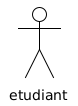
\includegraphics[width=.15\linewidth]{actor}
			\caption{Un acteur en UML}
			\label{fig:sub1}
		\end{subfigure}%
		\begin{subfigure}{.5\textwidth}
			\centering
			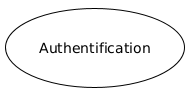
\includegraphics[width=.4\linewidth]{use_case}
			\caption{Un cas d'utilisatin en UML}
			\label{fig:sub2}
		\end{subfigure}
		\caption{Acteur et Use case en UML}
		\label{fig:figure1}
	\end{figure}

	\textbf{Acteurs \& Cas d'utilisations}
	
	Avant de pouvoir utiliser la plateforme, chaque utilisateur devra d'abord s'authentifier.	Le cas d’utilisation S'authentifier est une condition sine qua non pour pouvoir profiter pleinement des fonctionnalités du système.
	Dans le système qui sera mis en place, on aura les acteurs et leurs use case suivants :
	\begin{enumerate}
		\item l'étudiant :
		\begin{itemize}
			\item S'inscrire
			\item Gérer CompteInscription : Annuler, Modifier
			\item Demande Certificat 
		\end{itemize}
		%\item l'enseignant 
		\item la scolarité :
		\begin{itemize}
			\item Gérer Inscription : Enregistrer, Modifier, Supprimer 
			\item Gérer Certificat 
		\end{itemize}
		\item le décanat :
		\begin{itemize}
			\item Gérer Matricule : Attribuer, Modifier
			\item Gérer Carte 
		\end{itemize}
		\item l'administrateur :
		\begin{itemize}
			\item Gérer Compte : Créer, Modifier, Supprimer, Gérer Droit
			\item Parametrer la plateforme
		\end{itemize}
	\end{enumerate}
	
	On retient donc quatre utilisateurs qui sont entre autres l’étudiant, la scolarité, le décanat et l’administrateur. Chaque utilisateur a ses droit d’accès et ses fonctionnalités qui lui sont spécifiques pour des raisons de sécurité d’intégrité. Donc l'acteur administrateur comme son nom l’indique est l'utilisateur \textit{root} du système du faite qu'il possède tous les droits d'accès au système.
	
	La figure \ref{fig:figure3} repésente le diagramme de cas d'utilisation du système dans lequel on y voit clairement les différents acteurs et leurs cas d'utilisations.
	
	\begin{figure}[H]
		\centering
		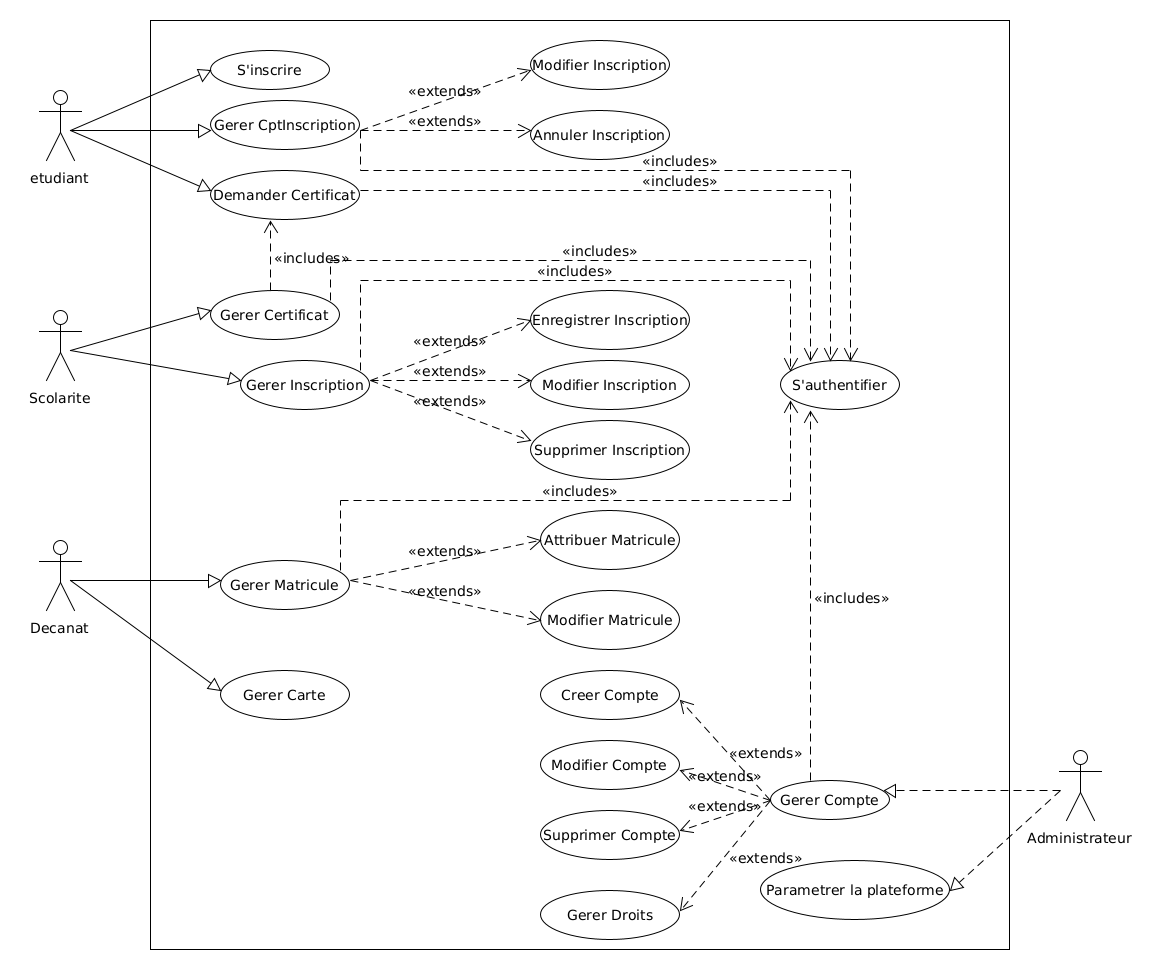
\includegraphics[width=\textwidth]{use_case_diag}
		\caption{Diagramme des cas d'utilisation}
		\label{fig:figure3}
	\end{figure}

	%\textbf{Description des cas d'utilisations}

	\subsubsection{Diagramme de classe}
	Le diagramme de classes décrit la structure interne du système
	modélisé i.e. ce qui doit être présent. Il décrit le système en
	visualisant les différents types d‘objets au sein du système et
	les types de relations statiques qui existent entre eux. Il illustre
	également les opérations ainsi que les attributs des classes. Un objet est une entité concraite ou abstraite du domaine
	d’application qui est décrite par une adresse mémoire, des
	attributs et opérations (méthodes et fonctions). C’est
	l’instance d’une classe. Une classe est un régroupement d’objets de même nature i.e.	un ensemble d’objet ayant les même attributs et les même
	opérations.
		
	Les différentes classes du système sont :
	\begin{itemize}
		\item Etudiant
		\item Dossier
		\item Quittus
		\item Matiere
		\item Composition
		\item Filiere
		\item Departement
		\item Faculte
		\item Scolarite
		\item Decanat
	\end{itemize}
	
	En UML, Une classe est représentée par un rectangle séparé en trois parties :
	\begin{itemize}
		\item la première partie contient le nom de la classe
		\item la seconde contient les attributs de la classe
		\item la dernière contient les méthodes de la classe
	\end{itemize}
	La seconde et la dernière représentent le comportement de la classe.
	\begin{figure}[H]
		\centering
		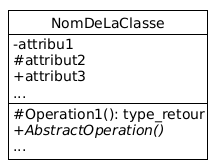
\includegraphics[width=.25\textwidth]{class}
		\caption{Une classe en UML}
		\label{fig:figure2}
	\end{figure}

	Le diagramme de classe est d'une grande utilité car il permet de modéliser les objets qui constituent le système, d'afficher les relations existante entre les objets et de décrire ce qu’ils font et les services qu’ils fournissent. Aussi, il permet de visualiser, définir et documenter des fonctions structurelles dans nos modèles.\\
	Le diagramme de classe suivant (Figure \ref{fig:figure4}) montre, les différentes classes du système ainsi que les relations qui existes entre elles et leurs multiplicité.
	
	\begin{figure}[H]
		\centering
		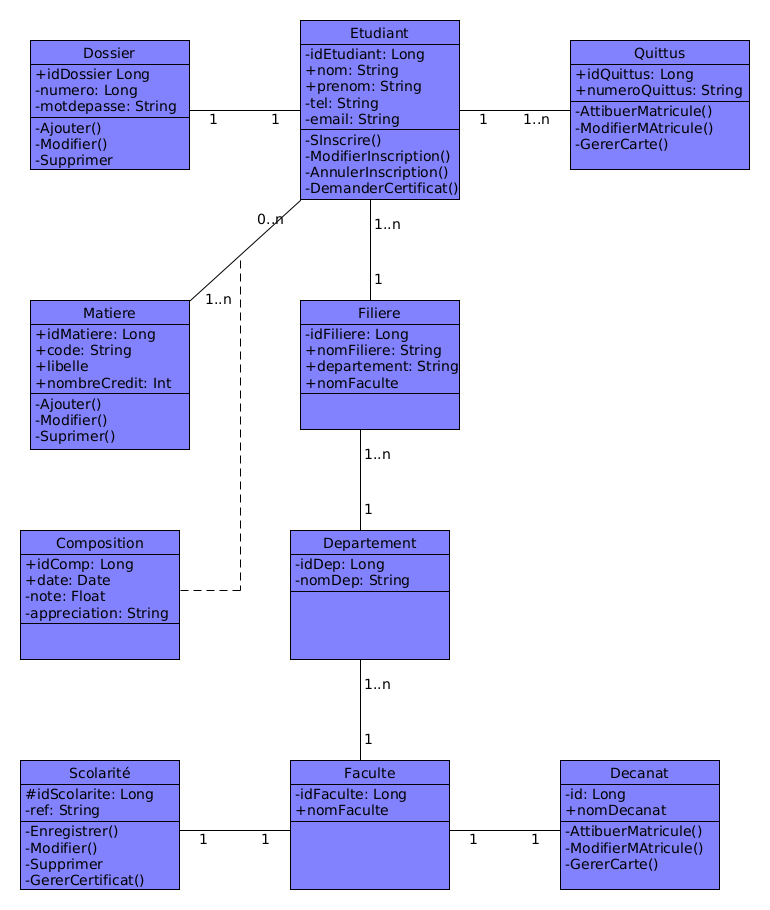
\includegraphics[width=\textwidth]{u_class_diag_1}
		\caption{Diagramme des classe}
		\label{fig:figure4}
	\end{figure}

	\newpage
	\subsection{MERISE}
	MERISE est une méthode d’analyse, de conception et de gestion de projets informatiques. Elle a pour but de concevoir des systèmes d’information et est basée sur la séparation des données et des traitements en plusieurs modèles conceptuels et physiques.
	
	Pour l’analyse et la conception de notre système, on va modéliser les modèles suivants : le Modèle Conceptuel des données (MCD), le Modèle Logique des données (MLD) et le Modèle Physique des données (MPD). Cette liste n'est pas exhaustive mais s'interessera à ceux-ci pour le moment.\\


	\subsubsection{MCD}
	Appelé aussi Modèles Entités/Associations (E/A), le MCD a pour but d'écrire de façon formelle les données qui seront utilisées par le système d'information. Il s'agit donc d'une représentation des données, facilement compréhensible. Il permettant de décrire le système d'information en usant des entités et des associations.
	
	En MERISE, une entité est un ensemble d'objet appartenant à un même ensemble qui est représenté par un rectangle. Une association est un lien sémantiques qu'il entre des entités le plus souvent désigné par un verbe.
	
	\begin{figure}[H]
		\centering
		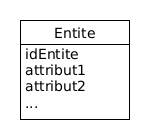
\includegraphics[width=.25\textwidth]{entite}
		\caption{Modélisation d'un Entité en MRISE.}
		\label{fig:figure5}
	\end{figure}

	\begin{figure}[H]
	\centering
	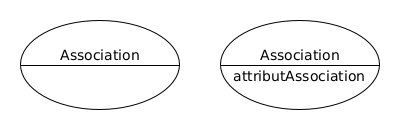
\includegraphics[width=.75\textwidth]{association}
	\caption{Représentation d'un Association et d'un Association ayant un attribut d'association en MERISE.}
	\label{fig:figure5.5}
	\end{figure}

	Les entités qui peuvent exister dans le système sont :
	\begin{itemize}
		\item Etudiant
		\item Dossier
		\item Quittus
		\item Matiere
		\item Filiere
		\item Departement
		\item Faculte
		\item Scolarite
		\item Decanat
	\end{itemize}
	Le tableau suivant liste les différentes associations et les entités respectives qu'elles relient :
	%Les associations reliant ces différentes entités sont illustrées dans le tableau suivant :
	\begin{table}[h!]
		\centering
		\begin{tabular}{|| c | c||}
			\hline 
			Associations & Entités concernées \\[0.5ex]
			\hline \hline
			DConcerner & \begin{tabular}{c}
				Etudiant \\ Dossier
			\end{tabular} \\
			\hline
			Retirer & \begin{tabular}{c}
				Etudiant \\ Dossier
			\end{tabular} \\
			\hline
			Composer & \begin{tabular}{c}
				Etudiant \\ Quittus
			\end{tabular} \\
			\hline
			SInscrire & \begin{tabular}{c}
				Etudiant \\ Matiere
			\end{tabular} \\
			\hline
			Apppartenir & \begin{tabular}{c}
				Etudiant \\ Filiere
			\end{tabular} \\
			\hline
			Contenir & \begin{tabular}{c}
				Filiere \\ Faculte
			\end{tabular} \\
			\hline
			SConcerner & \begin{tabular}{c}
				Faculte \\ Decanat
			\end{tabular} \\
			\hline
			Concerner & \begin{tabular}{c}
				Faculte \\ Scolarite
			\end{tabular} \\
			\hline
		\end{tabular}
		\caption{Entités et leurs Associations respectives.}
		\label{table:e_a}
	\end{table}
	
	\begin{figure}[H]
		\centering
		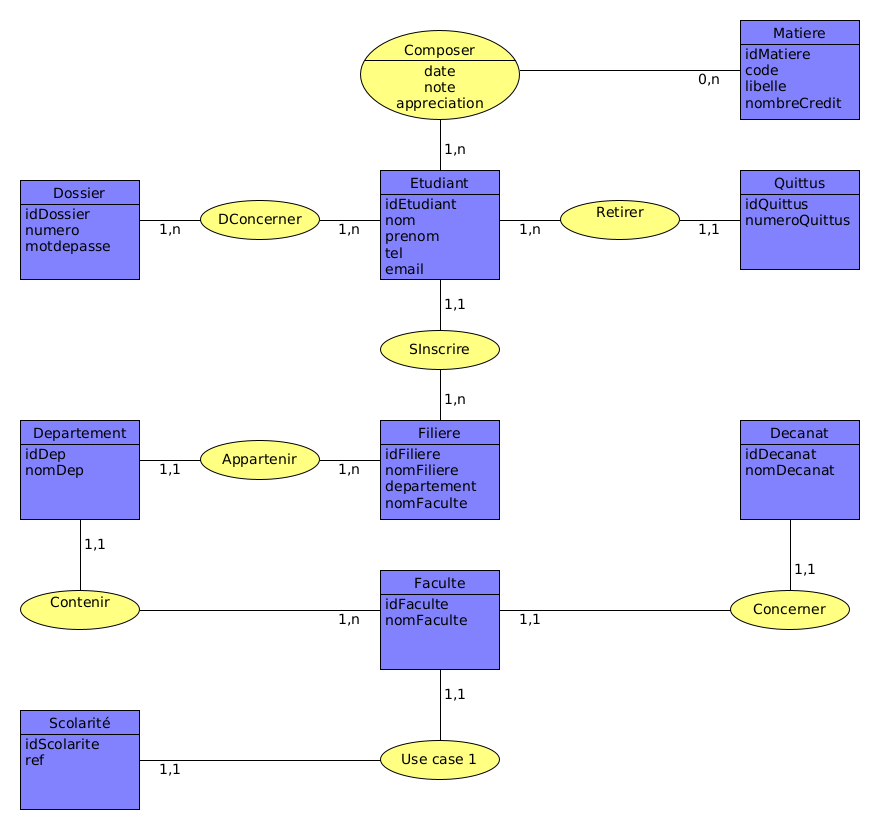
\includegraphics[width=\textwidth]{mcd}
		\caption{Modèle Conceptuel des Données}
		\label{fig:figure6}
	\end{figure}

	\subsubsection{MLD}
	Ce modèle consiste à décrire la structure de données utilisée sans faire référence à un langage de programmation. Il s'agit donc de préciser le type de données utilisées lors des traitements. Ce modèle est donc dépendant du type de base de données a utiliser.
	Pour passer du MCD au MDL, il y a quelques règles de transformation à respecter :
	\begin{itemize}
		\item Chaque entité du MCD devient une table dans le MLD;
		\item L'identifiant de l'entité devient la clé primaire de la tableet ses propriétés standards deviennent des attributs (colonnes) de la table;
		\item La clé primaire de la table basée sur l'entité à cardinalité (x,n) migre en tant que clé étrangère vers la table basée sur l'entité à cardinalité (x,1);
		\item Chaque association (x,n)-(x,n) (plusieurs à plusieurs) devient une table dont la clé primaire est formé par la concaténation des clés qui font reférences aux tables qu'elle relie et ses éventuelles propriétés deviennent des attributs;
		\item Chaque association unaire disparaît, la clé primaire de chacune des tables devient clé étrangère de l'autre. Pour les associations (0,1)-(1,1), on duplique la clé de la table basée sur l'entité à cardinalité (0,1) comme clé étrangère dans la table basée sur l'entité à cardinalité (1,1);
	\end{itemize}

	\begin{figure}[H]
		\centering
		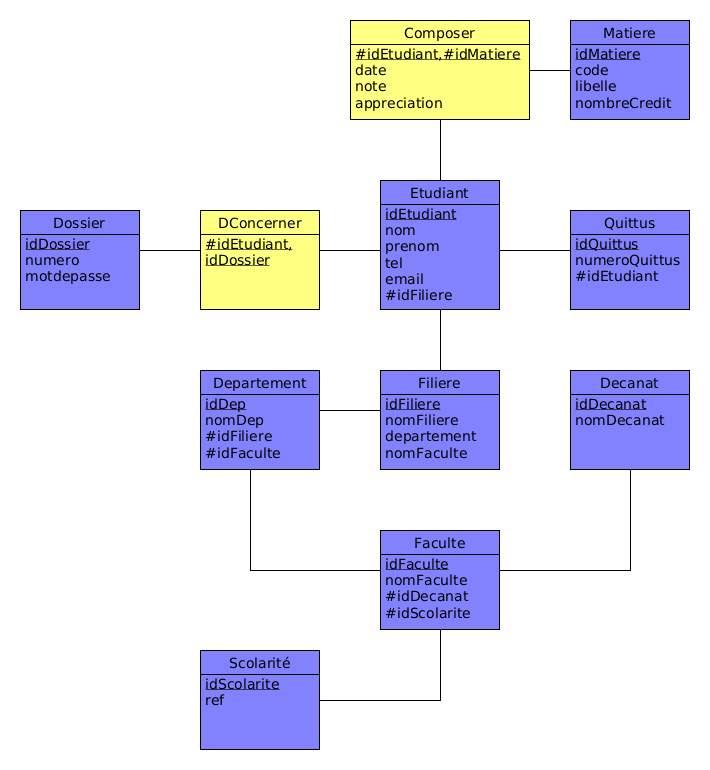
\includegraphics[width=\textwidth]{mld}
		\caption{Modèle Logique des Données}
		\label{fig:figure7}
	\end{figure}

	\subsubsection{MPD}
	Le MPD quand à lui consiste à implémenter le modèle dans le SGBD, c'est-à-dire le traduire dans un langage de définition de données. Dans cette étape, on utilise généralement le SQL.\\
	
	\newpage
	\section{Charte Graphique}
	La charte graphique définit les règles relatives à l'identité graphique d'un projet, d'une entreprise ou d'une organisation. Elle représente un élargissement de l'identité visuelle de l'entité au-delà des imprimés et de la signalétique pour englober les plateformes médiatiques et les signatures audio.
	
	\subsection{Police}
	Les police qui seront utilisées sont : \textbf{Sans} (Sans, Sans Bold, Sans ) et \textbf{DejaVu Sans Mono}.
	
	\subsection{Couleur}
	Les couleurs qui seront présentes sur la plateforme sont le blans, le bleu et le noir. Les texts sur fond blanc seront en noirs et les texts sur fond blue seront en blanc.
	
	\subsection{Logo}
	Le logo sera un avatar representant un étudiant.
	
	%\newpage
	%\section{Budget}
	
	%\newpage
	%\section{Delais d'Exécution}
	

	%\newpage
	%\section*{Conclusion}
	%\addcontentsline{toc}{section}{\protect\numberline{}Conclusion}
	
	\newpage
	\section*{Reférences}
	\addcontentsline{toc}{section}{\protect\numberline{}Reférences}
	Ci-dessous la list des liens de différentes pages web qui ont été consultées et la date de la dernière visite :
	\begin{itemize}
		\item \href{https://fr.wikipedia.org/wiki/Universit\%C3\%A9\_de\_N\%27Djam\%C3\%A9na}{https://fr.wikipedia.org/wiki/Universit\%C3\%A9\_de\_N\%27Djam\%C3\%A9na}, le 06 Février 2023
		\item \href{https://fr.wikipedia.org/wiki/Diagramme_de_cas_d\%27utilisation}{https://fr.wikipedia.org/wiki/Diagramme\_de\_cas\_d\%27utilisation}
		\item \href{https://fr.wikipedia.org/wiki/Charte_graphique}{https://fr.wikipedia.org/wiki/Charte\_graphique}
	\end{itemize}	
\end{document}